\section{Rules, Values and Conventions}\label{sec:rules}

\subsection{The Board and the Moves}
We play ordinary chess on the \emph{cylinder}, the $8\times8$ board with the a-file joined to the h-file. Only
the files wrap: ranks 1 and 8 are still edges. Every piece may cross the seam: a white pawn on h4 can capture on
a5, a knight on h1 gains a3 and b2, and a king on h1 gains a1 and a2, so a checkmate on the ordinary board need
not be one on the cylinder. A sliding piece stops before its ray returns to its own square, so a rook cannot
circle a rank as a null move. En passant (e.p.) is allowed, across the seam too. We write $\cyl{n}$ and
$\flatb{n}$ for the cylinder and the ordinary board with $n$ files and eight ranks.

\subsection{Notation}\label{sec:notation}
We use standard CGT notation~\cite{WinningWays,ONAG,Siegel2013}: $G=\game{G^L}{G^R}$ when white (Left)
can move to $G^L$ and black (Right) to $G^R$; in a sum $G+H$ the mover chooses one component; $G=H$ exactly
when $G-H$ is a second-player win, and every finite game has a unique \emph{canonical form}. The \emph{outcome class} is $\mathcal{L}$ or $\mathcal{R}$ if white or black wins whoever starts,
$\mathcal{N}$ if the first player wins and $\mathcal{P}$ if the second does. Our values include \emph{numbers}
(integers and dyadic fractions such as $1/2=\game{0}{1}$), \emph{switches} $\pm x=\game{x}{-x}$ with $x>0$
(sums are written without the plus sign, so $a\pm x=\game{a+x}{a-x}$), and \emph{nimbers}: in $\nim{k}$ either
player may move to any of $\nim{0}=0$, $\nim{1}=\star=\game{0}{0}$, \dots, $\nim{(k-1)}$, so
$\nim{2}=\game{0,\star}{0,\star}$. The \emph{birthday} of a game is the height of its canonical game tree, so
$\nim{k}$ has birthday $k$. Each game has a \emph{mean} and a \emph{temperature}, read from its
thermograph~\cite{WinningWays}; $\pm x$ has mean $0$ and temperature $x$. The \emph{left} and \emph{right stops}
are the numbers reached when white or black moves first and both play until a number appears. Infinitesimals
include \emph{up} ${\uparrow}=\game{0}{\star}$, ${\downarrow}=-{\uparrow}$, ${\Uparrow}={\uparrow}+{\uparrow}$,
and $\tinyg{1}=\ggame{0}{0\mid -1}=\game{0}{\game{0}{-1}}$.

\subsection{Normal Play and the Passed-Pawn Convention}
Following Elkies~\cite{Elkies1996}, we change chess just enough for normal play~\cite{WinningWays}. In pawn-only
positions a player who has no move loses; there are no null moves. A position in which exactly one side has a
passed pawn is decided, worth $+\BIG$ if that pawn is white and $-\BIG$ if it is black, where $\BIG$ exceeds the number of moves
either side can make (we use $\BIG=256$) and a pawn on its last rank counts as passed; M\"aser models such global threats with loopy
games~\cite{Maeser2002}. Kings are added as a group in mutual zugzwang, the tr\'ebuchet, and are then
\emph{frozen}: the model never moves them and counts the group as $0$, since whoever moves a king there first
loses a pawn, and then the game; Section~\ref{sec:kings} asks when this is exact. A move that gives both sides a
passed pawn makes a \emph{race position}, decided by one of three rules, none exact (a new queen may check or
stop the other pawn):
\begin{itemize}
\item \emph{count}: the side whose passed pawn needs fewer moves to promote wins, counting as on an empty
  board with a double step as one move; a tie goes to the side that did not move;
\item \emph{mover}: the side that made the move wins;
\item \emph{opponent}: the other side wins.
\end{itemize}

\subsection{En Passant and the Passed-Pawn Test}\label{sec:ep}
The textbook test calls a pawn passed if no enemy pawn stands ahead of it on its own file or a neighboring file
(on the cylinder, a and h are neighbors). En passant breaks this test: after a2--a4 in Fig.~\ref{fig:basic}(a)
the textbook test calls the a-pawn passed, yet black takes it en passant, b4$\times$a3. Elkies asked for a
more systematic treatment of en passant~\cite{Elkies1996}; we use a stricter test.

\begin{figure}[!t]
\centering
\begin{subfigure}[t]{0.32\columnwidth}\centering
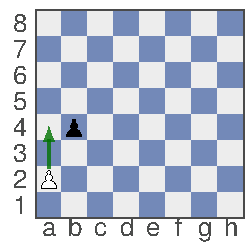
\includegraphics[width=\linewidth]{figures/ep_test.pdf}
\caption{\pos{W~a2 / B~b4}: $0$}
\end{subfigure}\hfill
\begin{subfigure}[t]{0.32\columnwidth}\centering
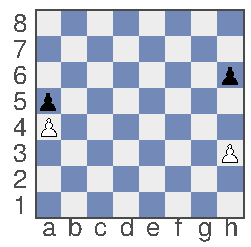
\includegraphics[width=\linewidth]{figures/zero_seam.pdf}
\caption{\pos{W~a4~h3 / \mbox{B~a5~h6}}: $0$}
\end{subfigure}\hfill
\begin{subfigure}[t]{0.32\columnwidth}\centering
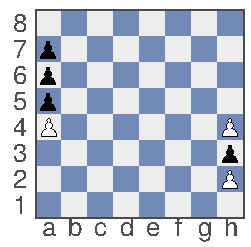
\includegraphics[width=\linewidth]{figures/tiny1_2025.pdf}
\caption{\pos{W~a4~h2~h4 / \mbox{B~a5~a6~a7~h3}}: $\tinyg{1}$}
\end{subfigure}
\caption{Basic positions. (a)~Ordinary board: after a2--a4 (arrow) the textbook test calls the a-pawn passed,
but b4$\times$a3 en passant removes it; under Definition~\ref{def:epaware} it is not passed. (b), (c)~Cylinder
(files a and h adjacent): a zero game and Tiny~1 that use the seam, in all nine settings. Positions of value
$1$, $2$, $\star$ and ${\uparrow}$ are in the supplementary material, Section~S1.}
\label{fig:basic}
\end{figure}

\begin{definition}[E.p.-aware passed pawn]\label{def:epaware}
A pawn is \emph{passed} if it passes the textbook test \emph{and} cannot be captured en passant on the
opponent's next move.
\end{definition}

One more white pawn makes the difference decisive. In \pos{W~a2~b3 / B~b4} black has no move, and the textbook
test lets white win at once with a2--a4. Under Definition~\ref{def:epaware}, every white move lets black capture
on a3, directly or en passant, and win the race that follows under the count rule, so the value is $0$. Across
the census of Section~\ref{sec:atlas} (at most six pawns, widths 1--4), the stricter test changes at least $18{,}137$ of the $231{,}071$ values,
$4{,}070$ of them in outcome \lab{C1} (Section~S1). The three race rules and three e.p.\ options
(textbook test, e.p.-aware test, e.p.\ off) give nine \emph{settings}. Values use the \emph{default setting}
(count rule, e.p.-aware test) unless stated.

\subsection{Components and the Cut Lemma}
A pawn changes file only by capturing onto a file where an enemy pawn stands (en passant included), so an empty
file stays empty forever and the pawns on either side of it never interact. Each block of neighboring occupied
files is a game of its own, a \emph{component}, and a position is the sum of its components; on the cylinder a
component is an arc or one \emph{ring} that uses every file.

\begin{theorem}[Cut lemma; \lab{P}, \lab{C2}]\label{thm:cut}
A pawn position on $\cyl{n}$ with at least one empty file has the same value as the position on
$\flatb{n-1}$ obtained by cutting the cylinder open along that file.
\end{theorem}

\begin{proof}
No pawn can move onto the empty file, so cutting the board there changes no legal move, no en passant right and
no passed-pawn test: the files beside the cut lose only a neighbor that stays empty forever.
\end{proof}

Hence values only a cylinder can make must come from rings (Section~\ref{sec:atlas}). A ring has no
empty file to separate a king group (Section~\ref{sec:kings-valid}), so ring values are pawn-model values only.

\section{Basic Positions on the Cylinder}\label{sec:basic}

The basic values of~\cite{Study2025} come from pawns alone. Each board in Fig.~\ref{fig:basic} leaves a file
empty, so by Theorem~\ref{thm:cut} its value is that of an ordinary-board position cut open along that
file~\cite{Elkies1996,WuYuLandry2010}, but the play crosses the seam. A move the opponent can answer with a
passed pawn loses and drops out~\cite{WinningWays,WuYuLandry2010}. The derivations of $1$, $2$, $\star$,
${\uparrow}$ and ${\Uparrow}\star$ are standard and are in Section~S1 of the supplementary material.

In Fig.~\ref{fig:basic}(b), if white goes first, it must play h3--h4, and black captures across the seam,
a5$\times$h4, with a passed pawn. If black goes first, h6--h5 is met by a4$\times$h5. Whoever moves first loses:
the value is $0$. Moving the white h-pawn back to h2 gives $1$, and moving the a-pawns up as well,
\pos{W~a5~h2 / B~a6~h7}, gives $2$, since black's h7--h5 is met by a5$\times$h6 en passant across the seam;
with e.p.\ off the value falls to the infinitesimal ${\Uparrow}\star$.

In Fig.~\ref{fig:basic}(c), white can take across the seam, h4$\times$a5, which leaves every pawn blocked: $0$.
White's h4--h5 drops out, since a6$\times$h5 wins for black. Black can only play a5$\times$h4; from there white
locks the a-file with a4--a5, leaving $0$, while black plays a6--a5 and keeps the spare move a7--a6, leaving
$-1$. So black's capture leads to $\game{0}{-1}=-\tfrac12\pm\tfrac12$, and $G=\tinyg{1}$, a positive
infinitesimal.
